%Note di Ingegneria del Software
%Sommario: Verifica e Validazione

\cornell{Verifica}{Accerta che l'esecuzione delle attività attuate nel periodo considerato non abbia introdotto errori \begin{itemize}
\item È un'attività continua
\item Si concentra sui processi
\item Eseguito ad ogni avanzamento intermedio meritevole di attenzione
\end{itemize}}

\cornell{Validazione}{Accerta che il prodotto sia conforme alle attese \begin{itemize}
\item Fatto \textbf{una volta solo} a fine progetto
\item "confronta" il prodotto finale con i requisiti
\item Si concentra sul prodotto
\end{itemize}}

\cornell{Forme Di Verifia}{\begin{itemize}
\item Analisi Statica
\begin{itemize}
\item Non richiede l'esecuzione del Software
\item Essenziale finchè il sistema non è completamente disponibile
\item Studia il codice e la documentazione
\item Verifica
        \begin{itemize}
                \item Conformità alle regole
                \item L'assenza di Difetti
                \item La presenza di proprietà positive
        \end{itemize}
\end{itemize}
\item Analisi Dinamica
        \begin{itemize}
                \item Richiede l'esecuzione del software
                \item Avviene tramite "test"
                \item Usata sia per verifica che validazione
        \end{itemize}
\end{itemize}}

\cornell{Verifica dell'analisi dei requisiti}{Fatta contro il capitolato ed il dominio del problema, richiede \begin{description}
                \item [Tracciabilità:] I requisiti derivano dal nulla, dal capitolato, dal dominio o dal proponente?
                \item [Regole per l'analisi:] Mi chiedo:
                        \begin{itemize}
                        \item Ho regole per l'analisi dei requisiti? Le ho applicate bene?
                        \item Ho una numerazione che classifica i requisiti in modo non ambiguo?
                        \item I requisiti sono associati alla fonte?
                        \item I requisiti sono associati al diagramma dei casi d'uso?
                        \item I requisiti sono chiari?
                        \item Ho trovato tutti i requisiti?
                        \item Ho capito bene i requisiti?
                \end{itemize}
                \end{description}
        Più prove trovo a favore dei vari requisiti, meglio è.
}

\cornell{Verifica della Progettazione}{\begin{description}
        \item [Per la progettazione logica] Viene fatta contro i requisiti, tramite regole definite
        \item [Per la progettazione di dettaglio] Viene fatta contro la progettazione logica
\end{description}
}

\cornell{Testing}{La "Validazione del Fornitore"\\
Analisi Dinamica\\
Ogni sezione di test deve subire analisi statica contro le sezioni di test precedenti}

\cornell{Unità}{Si definisce "unità" la più piccola quantità di Software: \begin{itemize}
        \item Verificabile \textbf{da solo}
        \item Prodotta dal singolo programmatore
        \item La definizione è sempre intesa in senso architetturale
        \item Non si tratta di linee di codice, ma di entità di organizzazione logica
\end{itemize}\\
Può essere vista come un compito assegnato ad un individuo, compreso completamente da tale individuo, verificabile singolarmente ed indipendentemente. Tale compito è portato a termine in breve tempo (solitamente nel giro di ore).\\
Prima di una commit, il codice deve passare i test di unità, quindi abbiamo una situazione in cui il programmatore può testare il proprio codice, anche se i testi sono scritti da altri.}

\cornell{Analisi Dinamica}{Se manca il main in una unità, vado a costruire un elemento detto "driver" (o "mock").\\
Se ho invece una componente all'interno dell'unità da testare che non voglio però che faccia parte del test, la sosituirò con uno "stub", che simula il comportamento di tale componente.\\
Driver e stub sono componenti "usa e getta".\\
Quindi formalmente: \begin{description}
        \item [Driver] Componente attiva fittizia che guida il test di una unità priva di main
        \item [Stub] Componente passiva fittizia per simulare una parte del sistema non oggetto del test
\end{description}\\
Inoltre è vitale dotarsi di un'ulteriore componente: \begin{description}
        \item [Logger] componente \textbf{non intrusiva} di registrazione dei dati d'esecuzione per analisi dei risultati
\end{description}}

\cornell{Esempio di Test}{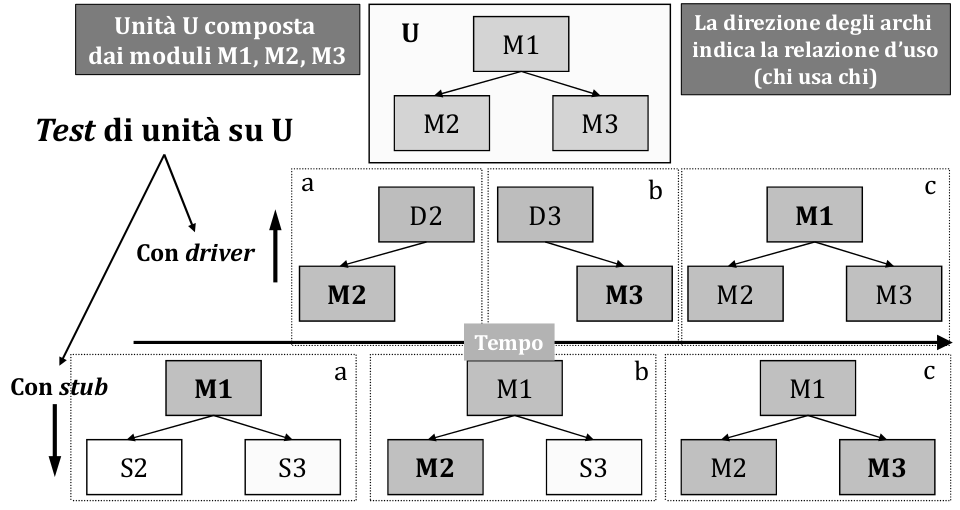
\includegraphics[scale=0.32]{images/60.png}}

\cornell{Tipi di Test}{\begin{itemize}
\item Test di Unità
\item Test di integrazione (tra le unità)
\item Test di Sistema
\item Test di regressione
\end{itemize}}

\cornell{Test di Unità}{Come tutti i test, Sono attività di analisi \textbf{ripetibili e deterministiche} \begin{itemize}
\item Col supporto di analisi statistica mirata
\item Si svolgono con massimo grado di parallelismo
\item Sono tanti, quindi vanno massimamente automatizzati
\item Vanno effettuati sotto condizioni controllate
\end{itemize}}

\cornell{Test di regressione}{Accertano che le modifiche fatte (che solitamente sono correttive) non facciano danno ad altri.\\
Quindi ogni parte P di S non deve causare errori in P od altre parti di S in relazione con P.\\
Vado a ripetere dei test già previsti ed effettuati per ogni P}

\cornell{Forme di Analisi Statica}{L'analisi statica si fa "leggendo"\\
La lettura è fatta in 2 forme: \begin{description}
        \item[Walkthrough] Attraversamento a pettine
        \item[Inspection] Osservazioni fatte sulla base di sospetti
\end{description}}

\cornell{Walkthrough}{\begin{itemize}
\item Cerca Difetti
\item Esegue una lettura Critica
        \begin{itemize}
                \item A largo spettro
                \item Senza l'assunzione di presupposti
        \end{itemize}
\item Fatta da gruppi misti di ispettori e sviluppatori con ruoli ben distinti, ed un arbitro
\item Per i listati di codice, vado a "simulare un'esecuzione"
\end{itemize}}

\cornell{Inspection}{\begin{itemize}
\item Cerca difetti
\item Esegue una lettura mirata, usando una checklist
\item Costa meno del walkthrough
\end{itemize}}

\cornell{Attività di Quality Assurance}{Raccolta di prove di qualità in maniera tempestiva \begin{itemize}
\item A fronte di metriche ed obiettivi definiti
\item Per controllo ed accertamento
\end{itemize}\\
Lo standard ISO/IEC 9126 è lo standard di riferimento per la qualità di prodotto.}
